% Three-column factor diagram for the A1-A4 (and A2/A4 targeted) framework:
%   Exposure Intensity  --x fully crossed-->  Exposure Item Type  --x fully crossed / 1-to-1-->  Outcome
%
% Build with:  tectonic publication/exposure_outcome_diagram.tex
% (or pdflatex if installed)

\documentclass[border=12pt, tikz]{standalone}

\usepackage{tikz}
\usetikzlibrary{positioning, decorations.pathreplacing, calc, arrows.meta, fit}

\begin{document}
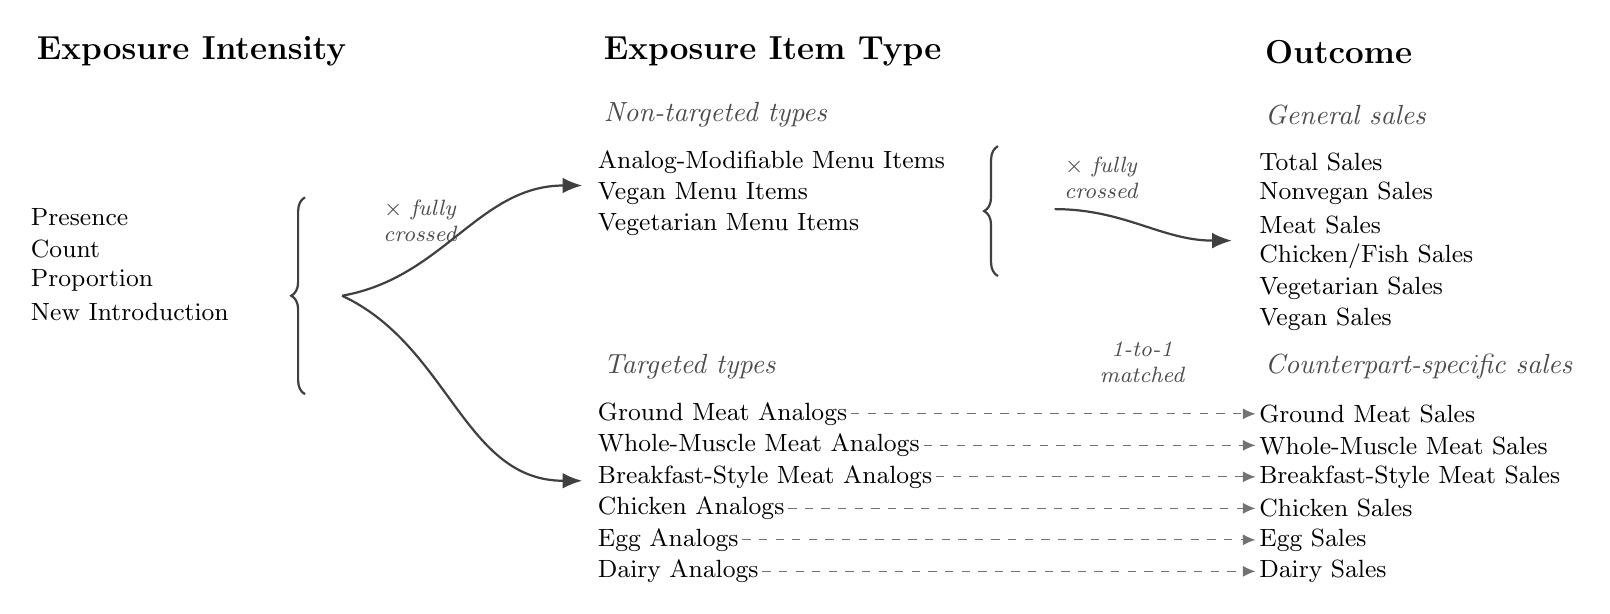
\begin{tikzpicture}[
  font=\small,
  col head/.style   = {font=\bfseries\large, anchor=west},
  block head/.style = {font=\itshape, anchor=west, text=black!70},
  item/.style       = {anchor=west, inner sep=1.2pt},
  arr/.style        = {-{Latex[length=2.5mm,width=2mm]}, thick, color=black!75},
  match/.style      = {-{Latex[length=1.6mm,width=1.4mm]}, thin, dashed, color=black!55},
  brace/.style      = {decorate, decoration={brace, amplitude=5pt, mirror, raise=2pt}, thick, color=black!75},
  cross/.style      = {font=\itshape\footnotesize, align=center, color=black!70, anchor=west},
]

% =============================================================
% Column 1 -- Exposure Intensity (4 rows)
% =============================================================
\node[col head]                  at (0, 5.4)  {Exposure Intensity};
\node[item] (c1a)                at (0, 3.3)  {Presence};
\node[item] (c1b) [below=4mm of c1a.west, anchor=west] {Count};
\node[item] (c1c) [below=4mm of c1b.west, anchor=west] {Proportion};
\node[item] (c1d) [below=4mm of c1c.west, anchor=west] {New Introduction};

% Right-side brace for column 1, with crossroad tip.
% Label is offset above-right of the tip so the diverging arrows don't pass through it.
\coordinate (c1bracetop) at (3.6, 3.55);
\coordinate (c1bracebot) at (3.6, 1.05);
\coordinate (c1tip)      at (4.0, 2.30);
\draw[brace] (c1bracetop) -- (c1bracebot);
\node[cross] at ($(c1tip)+(0.40,0.95)$) {$\times$ fully\\crossed};

% =============================================================
% Column 2 -- Exposure Item Type (two blocks)
% =============================================================
\node[col head]   at (7.2, 5.4)  {Exposure Item Type};

% Block 1: non-targeted types (3 rows)
\node[block head] at (7.2, 4.6)  {Non-targeted types};
\node[item] (c2a1) at (7.2, 4.0) {Analog-Modifiable Menu Items};
\node[item] (c2a2) [below=4mm of c2a1.west, anchor=west] {Vegan Menu Items};
\node[item] (c2a3) [below=4mm of c2a2.west, anchor=west] {Vegetarian Menu Items};

% Block 2: targeted types (6 rows)
\node[block head] at (7.2, 1.4)  {Targeted types};
\node[item] (c2b1) at (7.2, 0.8)  {Ground Meat Analogs};
\node[item] (c2b2) [below=4mm of c2b1.west, anchor=west] {Whole-Muscle Meat Analogs};
\node[item] (c2b3) [below=4mm of c2b2.west, anchor=west] {Breakfast-Style Meat Analogs};
\node[item] (c2b4) [below=4mm of c2b3.west, anchor=west] {Chicken Analogs};
\node[item] (c2b5) [below=4mm of c2b4.west, anchor=west] {Egg Analogs};
\node[item] (c2b6) [below=4mm of c2b5.west, anchor=west] {Dairy Analogs};

% Right-side brace for col 2 block 1 only (block 2 uses 1-to-1 dashed arrows,
% so an aggregate brace there would block the arrow paths).
\coordinate (c2top1) at (12.4, 4.20);
\coordinate (c2top2) at (12.4, 2.55);
\coordinate (c2top tip) at (12.95, 3.40);
\draw[brace] (c2top1) -- (c2top2);
\node[cross] at ($(c2top tip)+(0.10,0.40)$) {$\times$ fully\\crossed};

% Crossroad: arrows from col1 brace tip diverging to each col2 block
\draw[arr] (c1tip) to[out=10,  in=180] ($(c2a2.west)+(-0.15,0.1)$);
\draw[arr] (c1tip) to[out=-25, in=180] ($(c2b3.west)+(-0.15,-0.05)$);

% =============================================================
% Column 3 -- Outcome (two blocks)
% =============================================================
\node[col head]   at (15.6, 5.4)  {Outcome};

% Block 1: general sales (6 rows)
\node[block head] at (15.6, 4.6)  {General sales};
\node[item] (c3a1) at (15.6, 4.0) {Total Sales};
\node[item] (c3a2) [below=4mm of c3a1.west, anchor=west] {Nonvegan Sales};
\node[item] (c3a3) [below=4mm of c3a2.west, anchor=west] {Meat Sales};
\node[item] (c3a4) [below=4mm of c3a3.west, anchor=west] {Chicken/Fish Sales};
\node[item] (c3a5) [below=4mm of c3a4.west, anchor=west] {Vegetarian Sales};
\node[item] (c3a6) [below=4mm of c3a5.west, anchor=west] {Vegan Sales};

% Block 2: counterpart-specific sales (6 rows, aligned y with col 2 block 2)
\node[block head] at (15.6, 1.4)  {Counterpart-specific sales};
\node[item] (c3b1) at (15.6, 0.8)  {Ground Meat Sales};
\node[item] (c3b2) [below=4mm of c3b1.west, anchor=west] {Whole-Muscle Meat Sales};
\node[item] (c3b3) [below=4mm of c3b2.west, anchor=west] {Breakfast-Style Meat Sales};
\node[item] (c3b4) [below=4mm of c3b3.west, anchor=west] {Chicken Sales};
\node[item] (c3b5) [below=4mm of c3b4.west, anchor=west] {Egg Sales};
\node[item] (c3b6) [below=4mm of c3b5.west, anchor=west] {Dairy Sales};

% Single arrow from col2-block1 tip into col3-block1 (fully crossed)
\draw[arr] ($(c2top tip)+(0.10,0)$) to[out=0, in=180] ($(c3a3.west)+(-0.30,-0.20)$);

% 1-to-1 dashed matched arrows from col2-block2 to col3-block2
% Add a small label in the gutter to mark the 1-to-1 mapping.
\foreach \i in {1,...,6} {
  \draw[match] (c2b\i.east) -- (c3b\i.west);
}
% 1-to-1 label in the gutter between col2 and col3, lifted clear of the first dashed line
\node[cross] at (13.5, 1.45) {1-to-1\\matched};

\end{tikzpicture}
\end{document}
